\chapter{Developer Knowledge Classification}
\label{chap:experience}

In the previous chapters, I proposed that communication between notifications and developers could be improved if the information provided by notifications could adapt to the developer based on the developer's knowledge. 	
For it to be possible to adapt the information provided by notifications, tools need a way of knowing what concepts the developer knows and does not know. Furthermore, tools also need a way of knowing how well developers know these concepts. 	

In Chapter~\ref{chap:assess}, I outlined an approach for assessing developer knowledge of programming concepts. However, it is impractical and possibly infeasible to create a concept inventory for every programming concept and then ask developers to take that inventory before or while using a tool. It would be more practical and feasible if there was a way to use information already available to represent developer knowledge. I propose using developer experiences, in the form of the code they have written, to represent their knowledge of programming concepts. For the remainder of this document, I will refer to knowledge of programming concepts as \textit{conceptual knowledge}.  

Perception of any information provided to a developer is affected by that developer's knowledge and experiences; as a software developer, much of the knowledge accrued comes from experiences writing and modifying source code~\cite{Canas:1994:Mental,raju1995differential,fritz2010degree,argote2011organizational}.

However, currently tools have no way of assessing anything about the developer's knowledge.
Existing work in the area of source code mining has focused on measuring and predicting functional and non-functional properties of software~\cite{heckman2009model,menzies2007data,haapio2011exploring}. 
Contrary to much of the work in this area, I used source code mining to predict developer knowledge of programming concepts.

Based on previous research that suggests I can use source code as an indicator of how much a developer knows about a codebase~\cite{fritz2010degree}, I believe source code can also be an indicator of what developers know about programming.
Therefore, I designed a study to answer the following research questions:

\begin{itemize}
	\item [RQ\textsubscript{1}]: \textit{Is source code a good predictor of how much developers know about programming concepts?}
	\item [RQ\textsubscript{2}]: \textit{Does concept-specific source code increase the ability to classify how much developers know about programming concepts in comparison to a naive model?}
\end{itemize}

To answer these questions, I built and evaluated models that classify developers' conceptual knowledge. To determine if source code is a good predictor, I compared these models to random chance and a naive model that uses all the source code written by the developer (LOC).
The assumption is that if my models can classify developers with greater than 50\% accuracy, they perform better than random chance.
I collected source code relevant to the Java programming concepts of variables, exception handling, and generics from 19, 35, and 23 developers, respectively. 
I distributed the concept inventories described in Chapter~\ref{chap:assess} to validate conceptual knowledge for each model. 
I trained each model using source code the developers wrote pertaining to each programming concept, or \textit{concept-specific code}, in public GitHub repositories. 
I used unsupervised learning to determine a model that classifies developers based on their conceptual knowledge. 
Specifically, I calculated model metrics, such as precision, recall, and false positive rate, to determine and compare model performance.

% TODO make sure each chapter has contribution(s) listed -- a summary like this at the end of each chapter intro would be nice	
The contribution of this chapter is a validated approach and set of models for predicting developer conceptual knowledge using public developer source code contributions. For RQ\textsubscript{1}, I found that models using source code outperformed a model that randomly assigns developers' expertise. For RQ\textsubscript{2}, I found that concept-specific models outperformed models that attempt to assign expertise based on total lines of code (LOC) written.

\section{Knowledge Acquisition}
% TODO do I need to expand on this more?
According to existing research, we acquire knowledge through our experiences~\cite{argote2011organizational}. For example, a chef's knowledge regarding recipes, best practices, and what tastes good comes from their experiences cooking in both professional and informal settings. Just as a chef gains knowledge from her experiences, as do other professions. Software development is no exclusion.

Much of what software developers do involves looking at, writing, or modifying source code. 
There are a variety of other experiences that come with being a software developer. However, for scoping and proof-of-concept purposes, I focus on the primary task of software development which is writing code.
In the following section, I discuss how I used concept inventories and developer source code contributions to classify developer based on their conceptual knowledge.

\section{Knowledge Classification}

To determine the ability to use developer source contributions to predict developer knowledge, I used concept inventories to validate developer knowledge and source code contributions on GitHub to predict validated knowledge classifications.
To explain the process used to validate and predict developer knowledge, I will use a hypothetical developer Gabrielle and her experiences writing code as an example.

\subsection{Knowledge Validation}

To determine ground-truth developer knowledge for the models, I borrowed from computer science education literature and developed a set of concept inventories~\cite{tew2010assessing}.
The process for creating and validating these inventories is discussed in detail in Chapter~\ref{chap:assess}.
The scores from the concept inventories provide data that I used to provide an independent attribute for each model. 

\subsection{Knowledge Prediction}
% process for predicting knowledge
The goal of this study was to determine the possibility of using developer source code contributions to predict how much they know about programming concepts in their tool notifications.
Using developer source code, along with their concept inventory scores and the independent attributes, I used unsupervised learning to determine the relationship between the two.

\begin{figure} [ht]
	\centering
	\includegraphics[width=4.5in]{Chapter-6/figs/approach-fig.pdf}
	\caption{An overview of my approach.}
	\label{fig:approach}
\end{figure}

\subsubsection*{Source Code Contributions} \label{subsec:code}

To determine the dependent attributes for each model, and answer \textbf{RQ\textsubscript{1}}, I analyzed developers' public repositories for code contributions and assigned them to developers using version control (Figure~\ref{fig:approach}b).

Consider the code in Figure~\ref{fig:code}, which is a portion of code from the JUnit4\footnote{\url{http://junit.org/junit4/}} repository. Gabrielle contributes to this repository often, which provides rich data regarding her experiences with programming concepts. I analyzed developer source code using the Eclipse JDT ASTParser~\cite{eclipseASTParser}. Analyzing code statically with the ASTParser detects the presence of concept-specific code. However, it cannot tell us who contributed that code. In order to predict individual developer knowledge, we need to be able to identify that developer's code contributions.

Therefore, I used code bases in repositories so we could determine what developer made what contribution via the commit history. Since I chose the versioning platform Git,\footnote{\url{https://git-scm.com/}} I used JGit\footnote{\url{http://eclipse.org/jgit/}}, a Java library that allows for manipulation of Git repositories via Java code. Also,  next to SVN, Git is one of the most popular versioning softwares in use today.\footnote{\url{http://www.openhub.net/repositories/compare}}  Along with using ASTParser, I used JGit to analyze for individual developer code contributions. 

Previous research suggests time may play a factor in how predictive code contributions can be~\cite{johnson2015bespoke}, therefore I also used JGit to detect when the most recent contribution of each type of concept usage was made.
We chose to use GitHub, a social coding site where developers can create and maintain Git repositories,\footnote{\url{http://www.github.com}} as the source of data because GitHub stores Git repositories and many repositories on GitHub are public.
Once a plan was in place for analyzing developers repositories, to answer RQ\textsubscript{1}, I next identify source code that is directly related to the programming concepts of interest. 

\newcolumntype{g}{>{\columncolor{gray!40}}l}

\begin{table*}
    \centering
	\caption{Source Code Collected for Variables}
	\label{tab:var_code}
	\def\arraystretch{1.2}
	
	\begin{tabular}{ggg}
	    \toprule
		\rowcolor{white}
		\textbf{Source Code}                     & \textbf{Description}                                          & \textbf{Example}   
		\\
		\midrule
		\rowcolor{white}
		\textit{Primitive Types}        & \begin{tabular}[c]{@{}l@{}}data type is one of the most basic  \\Java data types (i.e. \texttt{int}) and store \\a value.\textbf{$\star\star$} (\textbf{D})\end{tabular}                                        & \small{\texttt{int a = 3;}}                                                                  \\
		\textit{Non-Primitive Types}    & \begin{tabular}[c]{@{}l@{}}data type is a reference data type \\and stores a reference to an object.\textbf{$\star$} (\textbf{D})\end{tabular}          & \small{\texttt{Object o = new Object();}}                                                    \\
		\rowcolor{white}
		\textit{Fields}                 & \begin{tabular}[c]{@{}l@{}}created to be accessed globally \\ by a class.\textbf{$\star$} (\textbf{D}) \end{tabular}                                                                               & \small{\texttt{public String s;}}                                                            \\
		
		\textit{Local Variables}        & \begin{tabular}[c]{@{}l@{}}created and assigned a value to be accessed \\locally by a method or construct.\textbf{$\star\star$} (\textbf{D}) \end{tabular}     & \small{\texttt{public String s = "hi";}}                                                     \\
		\rowcolor{white}
		\textit{Parameters}             & \begin{tabular}[c]{@{}l@{}}used as parameters to pass information \\into a method the developer created.\textbf{$\star\star\star$} (\textbf{D})\end{tabular}       & \small{\texttt{public void foo (String s)}}                                                  \\
		\textit{Public Variables}       & includes the public modifier.\textbf{$\star\star$} (\textbf{D})                                                                                              & \small{\texttt{public String s = "hi";} }                                                    \\
		\rowcolor{white}
        \textit{Private Variables}      & includes the private modifier.\textbf{$\star\star$} (\textbf{D})                                                                                              & \small{\texttt{private String s = "hi";}}                                               \\
		 \textit{Protected Variables}    & includes the protected modifier.\textbf{$\star\star\star$} (\textbf{D})                                                                                          & \small{\texttt{protected String s = "hi";}}                                                  \\
		\rowcolor{white}
		\textit{Static Variables}       & includes the static modifier.\textbf{$\star\star$} (\textbf{D})                                                                                              & \small{\texttt{static String s = "hi";}}                                              \\
		\textit{Final Variables}        & includes the final modifier.\textbf{$\star\star\star$} (\textbf{D})                                                                                                & \small{\texttt{final String s = "hi";}}                                               \\
		\rowcolor{white}
		\textit{Transient Variables}    & includes the transient modifier.\textbf{$\star\star\star$} (\textbf{D})                                                                                            & \small{\texttt{transient String s = "hi";}}                                           \\
		\textit{Volatile Variables}     & includes the volatile modifier.\textbf{$\star\star\star$} (\textbf{D})                                                                                           & \small{\texttt{volatile String s = "hi";}   } 
		\\
		\bottomrule
	\end{tabular}
	
\end{table*}

\begin{table*}
    \centering
	\caption{Source Code Collected for Exceptions}
	\label{tab:excep_code}
	\def\arraystretch{1.2}
	\begin{tabular}{ggg}
	\toprule
	\rowcolor{white}
		\textbf{Source Code}                     & \textbf{Description}                               & \textbf{Example}                                                                     \\
		\midrule
		\rowcolor{white}
		\textit{Throws Methods}         & \begin{tabular}[c]{@{}l@{}}method that throws an \\exception in the signature.\textbf{$\star$} (\textbf{U}) \end{tabular}                                & \begin{tabular}[c]{@{}l@{}}\small{\texttt{public void foo() }} \\\small{\texttt{throws IOException} }    \end{tabular}                                   \\
		\textit{Try Statements}         & non-empty try block.\textbf{$\star\star$} (\textbf{U})                                                                                                        & \small{\texttt{try \{ ... \}}}                                                               \\
		\rowcolor{white}
		\textit{Catch Blocks}           & non-empty catch block.\textbf{$\star$} (\textbf{U})                                                                                                      & \small{\texttt{catch (IOException e)\{...\}}}                                                \\
		\textit{Multi-Catch Blocks}     & \begin{tabular}[c]{@{}l@{}}non-empty catch block \\that use the  multi-catch \\operator ( $\vert$ ).\textbf{$\star\star\star$} (\textbf{U})\end{tabular}             & \begin{tabular}[c]{@{}l@{}}\small{\texttt{catch (IOException }} \\\small{\texttt{| SecurityException e) }}\end{tabular}
		\\
		\rowcolor{white}
		\textit{Try-With-Resources}     & \begin{tabular}[c]{@{}l@{}}non-empty try block that \\uses the try-with-resources \\feature.\textbf{$\star\star\star$} (\textbf{U})\end{tabular}                    & \begin{tabular}[c]{@{}l@{}}\small{\texttt{try (BufferedReader br =}} \\ \small{\texttt{new BufferedReader())}} \end{tabular}          
		\\
		\textit{Finally Blocks}         & non-empty finally block.\textbf{$\star\star\star$} (\textbf{U})                                                                                                 &  \small{\texttt{finally \{...\}}}                                                                           \\
	    \rowcolor{white}
	    \textit{Throw Statements}       & \begin{tabular}[c]{@{}l@{}}statement in method body \\that throws an exception.\textbf{$\star\star$} (\textbf{U}) \end{tabular}                               & \small{\texttt{throw new IOException();}}                                                    \\
		\textit{Exception Declarations} & \begin{tabular}[c]{@{}l@{}}creation of a new exception \\class.\textbf{$\star\star$} (\textbf{D}) \end{tabular}                                                                                        & \begin{tabular}[c]{@{}l@{}}\small{\texttt{public class NewException}} \\\small{\texttt{extends Exception}}   \end{tabular}                     \\
		\rowcolor{white}
		\textit{Catch Exceptions}       & \begin{tabular}[c]{@{}l@{}}non-empty catch blocks that \\catch the generic Exception.\textbf{$\star\star$} (\textbf{U}) \end{tabular}                         & \small{\texttt{catch (Exception e) \{...\} }  }                                              \\
		\textit{Checked Exceptions}     & \begin{tabular}[c]{@{}l@{}}statement that uses exceptions \\that are checked at compile\\-time.\textbf{$\star$} (\textbf{U})\end{tabular}                & \small{\texttt{FileNotFoundException}}                                                       \\
		\rowcolor{white}
		\textit{Unchecked Exceptions}   & \begin{tabular}[c]{@{}l@{}}statement that uses exceptions \\that are not checked at \\compile-time.\textbf{$\star\star$} (\textbf{U}) \end{tabular}             & \small{\texttt{RuntimeException}}                                                            \\
		\bottomrule
	\end{tabular}
\end{table*}

\begin{table*}
	\centering
	\caption{Source Code Collected for Generics}
	\label{tab:gen_code}
	\def\arraystretch{1.2}
	\begin{tabular}{ggg}
	\toprule
		\rowcolor{white}
		\textbf{Source Code}                     & \textbf{Description}                                    & \textbf{Example}      
		    \\
		\midrule
		\rowcolor{white}
        \begin{tabular}[c]{@{}l@{}}\textit{Type Argument} \\\textit{ Methods}\end{tabular}  & \begin{tabular}[c]{@{}l@{}}method with generic type \\argument(s).\textbf{$\star$} (\textbf{U})  \end{tabular}                                                                                     & \small{\texttt{public List<String> foo()}}                                
        \\
	    \textit{Wildcard Generics}      & \begin{tabular}[c]{@{}l@{}}usage of the wildcard type \\parameter.\textbf{$\star\star$} (\textbf{D}) \end{tabular}                                                                                    & \small{\texttt{List<?> String}}                                          
	    \\
		\rowcolor{white}
		\begin{tabular}[c]{@{}l@{}}\textit{Generic Type} \\\textit{ Declarations} \end{tabular} & \begin{tabular}[c]{@{}l@{}}creation of new generic \\class.\textbf{$\star$} (\textbf{D})     \end{tabular}                                                                                         & \small{\texttt{public class Bar<T>}}                                     
		\\
		\begin{tabular}[c]{@{}l@{}}\textit{Type Parameter} \\\textit{Fields} \end{tabular} & \begin{tabular}[c]{@{}l@{}}field with generic type \\parameter(s).\textbf{$\star\star$} (\textbf{D})  \end{tabular}                                                                                     & \small{\texttt{List<T> list;}}                                            
		\\
		\rowcolor{white}
		\begin{tabular}[c]{@{}l@{}}\textit{Type Parameter} \\\textit{Method} \end{tabular} & \begin{tabular}[c]{@{}l@{}}method with generic type \\parameter(s).\textbf{$\star\star$} (\textbf{D})   \end{tabular}                                                                                   & \small{\texttt{public List<T> foo()} }                                    
		\\
		\textit{Diamond Generics}       & \begin{tabular}[c]{@{}l@{}} usage of the diamond \\operator.\textbf{$\star\star\star$} (\textbf{U}) \end{tabular}                                                                                            & \small{\texttt{... = new List<>();}}                                      
		\\
		\rowcolor{white}
		\begin{tabular}[c]{@{}l@{}}\textit{Explicit Method} \\\textit{Invocation} \end{tabular}  & \begin{tabular}[c]{@{}l@{}}method invocation with \\explicit generic type \\arguments.\textbf{$\star\star\star$} (\textbf{U}) \end{tabular}                       & \small{\texttt{Collections.<Number, Long>collect(...)} }                  
		\\
		\begin{tabular}[c]{@{}l@{}}\textit{Implicit Method} \\\textit{Invocation}  \end{tabular} & \begin{tabular}[c]{@{}l@{}}method invocation with \\implied generic type \\arguments.\textbf{$\star$} (\textbf{U}) \end{tabular}                           & \small{\texttt{Collections.collect(...)} }                                                    
		\\
		\rowcolor{white}
		\begin{tabular}[c]{@{}l@{}}\textit{Generic Class} \\\textit{Instantiation} \end{tabular}&  \begin{tabular}[c]{@{}l@{}}instantiation of a generic \\class.\textbf{$\star$} (\textbf{U})  \end{tabular}      & \small{\texttt{Bar<String> b = new Bar<String>();} }   
		\\
	    \textit{Nested Generics}        & \begin{tabular}[c]{@{}l@{}}usage of generics within a \\generic construct.\textbf{$\star$} (\textbf{U}) \end{tabular}                                                                              & \small{\texttt{Map<Integer, List<String>> map = ...;}} \\
		\rowcolor{white}
		\begin{tabular}[c]{@{}l@{}}\textit{Bounded Type} \\\textit{Parameters} \end{tabular}  & \begin{tabular}[c]{@{}l@{}}generics with type \\bounds.\textbf{$\star\star\star$}  (\textbf{D}) \end{tabular}                                                                                               & \small{\texttt{List<T extends String> list;}}                             \\
		\bottomrule
	\end{tabular}
\end{table*}

\begin{figure} [ht]
	\centering
	\includegraphics[width=4.5in]{Chapter-6/figs/code.pdf}
	\caption{Mapping of developer source code contributions on one class in an open source repository.}
	\label{fig:code}
\end{figure}

\subsubsection{Concept-Specific Source Code}

To answer RQ\textsubscript{2}, I collected concept-specific code and manually collected lines of code (LOC) added to each repository for each developer from GitHub. 
I define concept-specific source code as code that, according to on-line resources, is relevant to understanding and using the concept in source code. 
Since much of a developer's experience is writing source code, and experience informs knowledge~\cite{bromme1995fusing,argote2011organizational}, I used total LOC as the naive model.

I used the same key concepts identified for the concept inventories to determine what concept-specific code to analyze for. 
For each concept, I used the same resources used to create the concept inventories to determine relevant code to collect from developers' repositories.
In the end, I collected 11 examples of generics usage, 10 examples of exception handling usage, and 12 examples of variables usage.\footnote{The repository that holds the analyzer used can be found at: www.github.com/brittjay0104/APATIANproto} All of the code I collected, along with a description and example for each, is shown in Tables~\ref{tab:var_code}--~\ref{tab:gen_code}. 
I manually checked the added lines reported by GitHub on each developer's repositories to determine LOC for the naive model.

Because Gabrielle took the variables and generics concept inventories, I analyzed her repositories for code that she contributed that related specifically to variables and generics. For example, looking at the code in Figure~\ref{fig:code}, in the class \texttt{LoggerRegistry<T extends ExtendedLogger>}, Gabrielle contributed both variables (lines 5 and 13) and generics code (lines lines 5, 13, and 23). 

The output of the analyzer for each repository is an occurrence count for all contributed concept-specific code and when the most recent contribution for each occurred.
For example, looking at Gabrielle's contributions in \texttt{LoggerRegistry<T extends ExtendedLogger>}, Gabrielle added two variables (a private final field at line 5 and a final parameter at line 13). For each variable she contributed, the analyzer would also note that her most recent contribution for each was in the past couple months.
Prior to dividing the data by features or applying heuristics, I used the list of concept-specific source code outlined in Table~\ref{tab:var_code} (Variables), Table~\ref{tab:excep_code} (Exception Handling), and Table~\ref{tab:gen_code} (Generics) to determine levels of source code usage.

\subsubsection{Source Code Usage Hierarchy}
I analyzed data from 19, 35, and 23 GitHub developers for variables, exception handling, and generics (respectively).
I used all the output from analyzing developers' code repositories to determine which types of concept usage might be more advanced than others. 
Based on frequency of source code usage across repositories and developers for each concept (Figure~\ref{fig:code}), I created a hierarchy of source code usage that outlines what source code collected might be considered basic, intermediate, or advanced. 
Under the assumption that the more something is used the less difficult (and more foundational) it is, I determined which features fit into which category by observing what source code developers used most often versus source code developers use least often. 
For example, only 27\% on the source code we collected included Bounded Type Parameters (Figure~\ref{fig:code}) as opposed to the 99\% of source code included Generic Type Declarations. Therefore, I consider Type Declarations basic usage and Bounded Type Parameters advanced usage. 
I determined thresholds by a leap in the total count of source code usage of more than 100.	
An example concept source code usage hierarchy, along with a more detailed description of the creation process and usage, can be found on-line with the other materials.
% TODO this becomes an Appendix


\subsubsection{Data Features and Heuristics}\label{subsec:prep}

To provide a wider range of generalizable attributes for answer our research questions, I characterized the dependent attributes (Figure~\ref{fig:approach}c) for the models by grouping concept-specific code collected above based on features of the data. 

For example, a feature of type parameter fields and methods (Figure~\ref{fig:code}, lines 5 and 13) that groups them together is Gabrielle wrote new generic code (Declarations) for use by other developers, rather than using existing generic code (Usages) as she did on line 23.
The set of features identified and used among the data are as follows:
\begin{itemize}
	\item \textbf{Levels of Concept Usage:} I computed the Levels of Concept Usage by adding together counts from the types of each concept that would be considered on a basic, intermediate, or advanced level of usage. I used the concept source code usage hierarchy discussed previously. 
	In Tables~\ref{tab:var_code}--~\ref{tab:gen_code}, Basic usage has one star (\textbf{$\star$}) at the end of its description, Intermediate two stars (\textbf{$\star\star$}), and Advanced three stars (\textbf{$\star\star\star$}).
	\item \textbf{Declarations:} I computed Declarations for each concept by adding together counts from the types of concept usage where the developer wrote new concept code for use by themselves or others (i.e. type declarations or new exception type). In Tables~\ref{tab:var_code}--~\ref{tab:gen_code}, Declarations are labeled with a \textbf{(D)} at the end of the description.
	\item \textbf{Usages}: We computed Usage by adding together counts from the types of concept usage where the developer is using code someone else wrote (i.e. method invocations), as opposed to contributing to a new type. In Tables~\ref{tab:var_code}--~\ref{tab:gen_code}, Usages are labeled with a \textbf{(U)} at the end of the description.
\end{itemize}

Because I currently only collect variable declarations, all variable concept-specific code collected for this study falls under Declarations.

Along with the above features, I also defined two heuristics to apply to the feature groups:

\begin{itemize}
	\item \textbf{Recency:} The recency heuristic takes each of the initial attribute values and multiplies each value by 1.0 if the most recent contribution was made in the last week, 0.8 if between one week and one month, 0.6 for 1--6 months, 0.4 for one year, and 0.2 for more than one year.
	For example, if, the total number of declarations made by the developer (Declaration heuristic) is 198 and the most recent declaration was written between one week and one month, the Type Declaration Recency (DeclRecency) heuristic value would be 158.4 (\(198 \times 0.8)\). 
	\item \textbf{Natural Log:} This heuristic calculates natural log of each feature group before and after the recency heuristic is applied.
\end{itemize}

I defined a recency heuristic because previous analyses suggested time may be a factor to consider when modeling knowledge~\cite{johnson2015bespoke}. 
For Gabrielle, if I only analyzed the class in Figure~\ref{fig:code}, Gabrielle contributed a field, private variable, final variable, and parameter; all would be assigned the same recency value (0.6) based on when she made the contribution(s).
Gabrielle contributed 3 pieces of generic code: a type parameter field (line 5), a type parameter method (line 13), and an implicit method invocation (line 23). However, as shown in Figure~\ref{fig:code}, Gabrielle contributed type parameter fields and methods more recently than she contributed implicit method invocations. Therefore, while Gabrielle's type parameter field and method recency value is 0.6, her implicit method invocation recency value would be 0.4.

I applied natural log to the data following the reasoning of Fritz and colleagues, who used natural log in their models to account for the potential for large differences in attribute values~\cite{fritz2010degree}. For example, some repositories returned counts in the thousands for class instantiations but counts of zero for explicit method invocations; this might cause the model to put more weight on the contribution of feature groups and heuristics that include class instantiations than it truly contributes.

\subsubsection{Developer Knowledge Classifications}
Once the attributes have been calculated, I performed discretization to convert the continuous concept inventory score values into intervals of values, or \emph{classes} (Figure~\ref{fig:approach}d)~\cite{fayyad1993multi}. This step became particularly important once I decided to use decision tree learners to answer the research questions -- I discuss the decision to use decision trees later in this section.

Discretization involves iteratively comparing attribute values for each instance and finding the ``best cut'' in the data; each cut is considered a class of the data. A distinguishing feature of this data set is its small size (just a few dozen rows). Hence, I cut the concept inventory scores for each model into two and three classes to answer the research questions. Two classes comes from cutting on the median. I chose three to account for the potential transition between classes~\cite{dreyfus2004five}. For the three way split, with the small data set, I tried to maintain relatively even size chunks while making sure there is some consistency across models (i.e. someone with a score of 7 or above is never a beginner).

The generics data yielded ternary discretization (three classes) and the variables and exceptions data yielded binary discretization (two classes). For data sets with three classes, I labeled each developer as either Beginner, Intermediate, or Expert. For data sets with two classes, I labeled each developer as either Beginner or Expert.	
Based on Gabrielle's concept inventory scores and source code data, she is labeled Expert for both generics and variables. 
We will talk about what the differences in the discretization output might mean in Section~\ref{sec:disc}.

\subsubsection{Attribute Selection}
Once I assigned classifications to each developer, I used developer knowledge classifications to perform Correlation-based Feature Selection (CFS) in Weka, software that provides a collection of machine learning algorithms for data mining~\cite{Hall:2009:WDM:1656274.1656278}. CFS helps to determine the attributes best suited for each model (Figure~\ref{fig:approach}e)~\cite{hall1999correlation} by pruning irrelevant attributes, leaving only the attributes that correlate the most with the developer's classification.

This analysis runs k-fold cross validation using the attributes passed in; to lower the potential for a model with overestimation bias, I maintained even and sizable chunks by using 4-fold cross validation.	
CFS evaluates each attribute on its predictive ability and uses cross-validation to indicate how stable the best subset of variables is based on how many folds the variable appeared in.
For increased model stability, I used the selection criteria that the attribute appear in two or more folds to be included in decision tree learning.

\subsubsection{Decision Tree Learning}
To answer the research questions, I used decision tree learning. 
More specifically, I used Weka's J48 classifier~\cite{witten1999weka} to create decision trees. 
Wolpert and colleagues~\cite{wolpert1997no} caution that one should not expect any particular algorithm to work best for all possible inputs. Hence, when exploring new data, is it necessary to conduct some experimentation to find useful settings for that data. Accordingly, I ran different analyses and learners to determine which learner was most effective for the data and research goals. Because there are so many machine learning algorithms availble, I neeeded to narrow down the learners I would experiment with. I chose to compare regression, Naive Bayes, and Decision Trees based on prior work with similar goals of making software development-related predictions~\cite{menzies2004assessing,menzies2007data,heckman2009model,fritz2010degree}. I found decision trees to be optimal for answering the research questions along with being more human readable.

Another motivation for using decision trees as opposed to regression or Naive Bayes is the relatively heightened error tolerance provided by decision tree learners. Because I only used public repository contributions, the data collected may have attributes with no data. For example, upon analyzing a developer's repositories I may find no occurrences of generic type declaration due to the fact that the developer has written generic type declarations in a context not being analyzed (i.e. local software projects). Using decision trees allows us to see meaningful relationships in the data, regardless of any data that may be erroneous or inaccurate.
% Based on the results from decision tree learning, I next .

\section{Knowledge Models}\label{sec:eval}

Based on developer classifications and the full set of attributes, CFS identified the following subset of attributes that fit my selection criteria:
\begin{itemize}
    \item \textbf{Variables} -- Public Variables
    \item \textbf{Exceptions} -- Advanced Exceptions, Try Statements Recency, Finally Blocks Recency, and Throws Methods
	\item \textbf{Generics} -- LOC, Generic Type Declarations, and Generic Type Declarations Recency
\end{itemize}

I created a decision tree model for each concept with all the concept-specific attributes above to answer RQ\textsubscript{1}. To answer RQ\textsubscript{2}, I created a LOC only model, when LOC met the attribute selection criteria, to compare to the concept-specific models.
The values for each model's \emph{precision}, \emph{recall}, \emph{F-Score}, \emph{TP (True Positive) Rate}, and \emph{FP (False Positive) Rate} are shown in Tables~\ref{tab:vars},~\ref{tab:exceptions},~\ref{tab:gen}, and~\ref{tab:loc}. The resulting decision trees can be found in Figures~\ref{fig:vars},~\ref{fig:excep}, and~\ref{fig:gen}.

\begin{table}
	\centering
	\caption{Variables Model Accuracy}
	\label{tab:vars}
	\begin{tabular}{llll}
		\toprule
		\multicolumn{4}{c}{\textbf{Public Variables}}                               \\
		\cmidrule(lr){1-4}
		& \textbf{Beginner} & \textbf{Advanced} & \textbf{Total} \\
		\midrule
		\textbf{Precision} & 0.571             & 0.667             & 0.627          \\
		\textbf{Recall}    & 0.500             & 0.727             & 0.632          \\
		\textbf{F-Score}   & 0.533             & 0.696             & 0.627          \\
		\textbf{TP Rate}   & 0.500             & 0.727             & 0.632          \\
		\textbf{FP Rate}   & 0.273             & 0.500             & 0.404   \\
		\bottomrule
		
	\end{tabular}
\end{table}

\begin{table}
	\centering
	\caption{Exceptions Model Accuracy}
	\label{tab:exceptions}
	\begin{tabular}{llll}
		\toprule
		\multicolumn{4}{c}{\textbf{\begin{tabular}[c]{@{}c@{}}Advanced, Try Statement Recency, \\ Finally Block Recency, Throws Method \end{tabular}}} \\
		\cmidrule(lr){1-4}
		& \textbf{Beginner}                 & \textbf{Advanced}                 & \textbf{Total}                 \\
		\midrule
		\textbf{Precision}                 & 0.789                             & 0.750                             & 0.771                          \\
		\textbf{Recall}                    & 0.789                             & 0.750                             & 0.771                          \\
		\textbf{F-Score}                   & 0.789                             & 0.750                             & 0.771                          \\
		\textbf{TP Rate}                   & 0.789                             & 0.750                             & 0.771                          \\
		\textbf{FP Rate}                   & 0.250                             & 0.211                             & 0.232                         \\
		\bottomrule
	\end{tabular}
\end{table}

\begin{table}
	\centering
	\caption{Generics Model Accuracy (Non-LOC)}
	\label{tab:gen}
	\begin{tabular}{lllll}
		\toprule
		\multicolumn{5}{c}{\textbf{Declarations and DeclRecency (Generics)}}                                                            \\
		\cmidrule(lr){1-5}
		& \textbf{Beginner} & \textbf{Intermediate} & \textbf{Advanced} & \textbf{Total} \\
		\midrule
		\textbf{Precision} & 0.667             & 0.727                 & 0.875             & 0.729          \\
		\textbf{Recall}    & 0.333             & 0.889                 & 0.875             & 0.739          \\
		\textbf{F-Score}   & 0.444             & 0.8                   & 0.824             & 0.715          \\
		\textbf{TP Rate}   & 0.333             & 0.889                 & 0.875             & 0.739          \\
		\textbf{FP Rate}   & 0.059             & 0.214                 & 0.133             & 0.146         \\
		\bottomrule
	\end{tabular}
\end{table}

\begin{table}
	\centering
	\caption{Generics Model Accuracy (LOC only)}
	\label{tab:loc}
	\begin{tabular}{lllll}
		\toprule
		\multicolumn{5}{c}{\textbf{LOC (Generics)}}                                                         \\
		\cmidrule(lr){1-5}
		& \textbf{Beginner} & \textbf{Intermediate} & \textbf{Advanced} & \textbf{Total} \\
		\midrule
		\textbf{Precision} & 0.5               & 0.636                 & 0.875             & 0.684          \\
		\textbf{Recall}    & 0.333             & 0.778                 & 0.875             & 0.696          \\
		\textbf{F-Score}   & 0.4               & 0.7                   & 0.875             & 0.683          \\
		\textbf{TP Rate}   & 0.333             & 0.778                 & 0.875             & 0.696          \\
		\textbf{FP Rate}   & 0.118             & 0.286                 & 0.067             & 0.166         \\
		\bottomrule
	\end{tabular}
\end{table}

\begin{figure} [h]
	\centering
	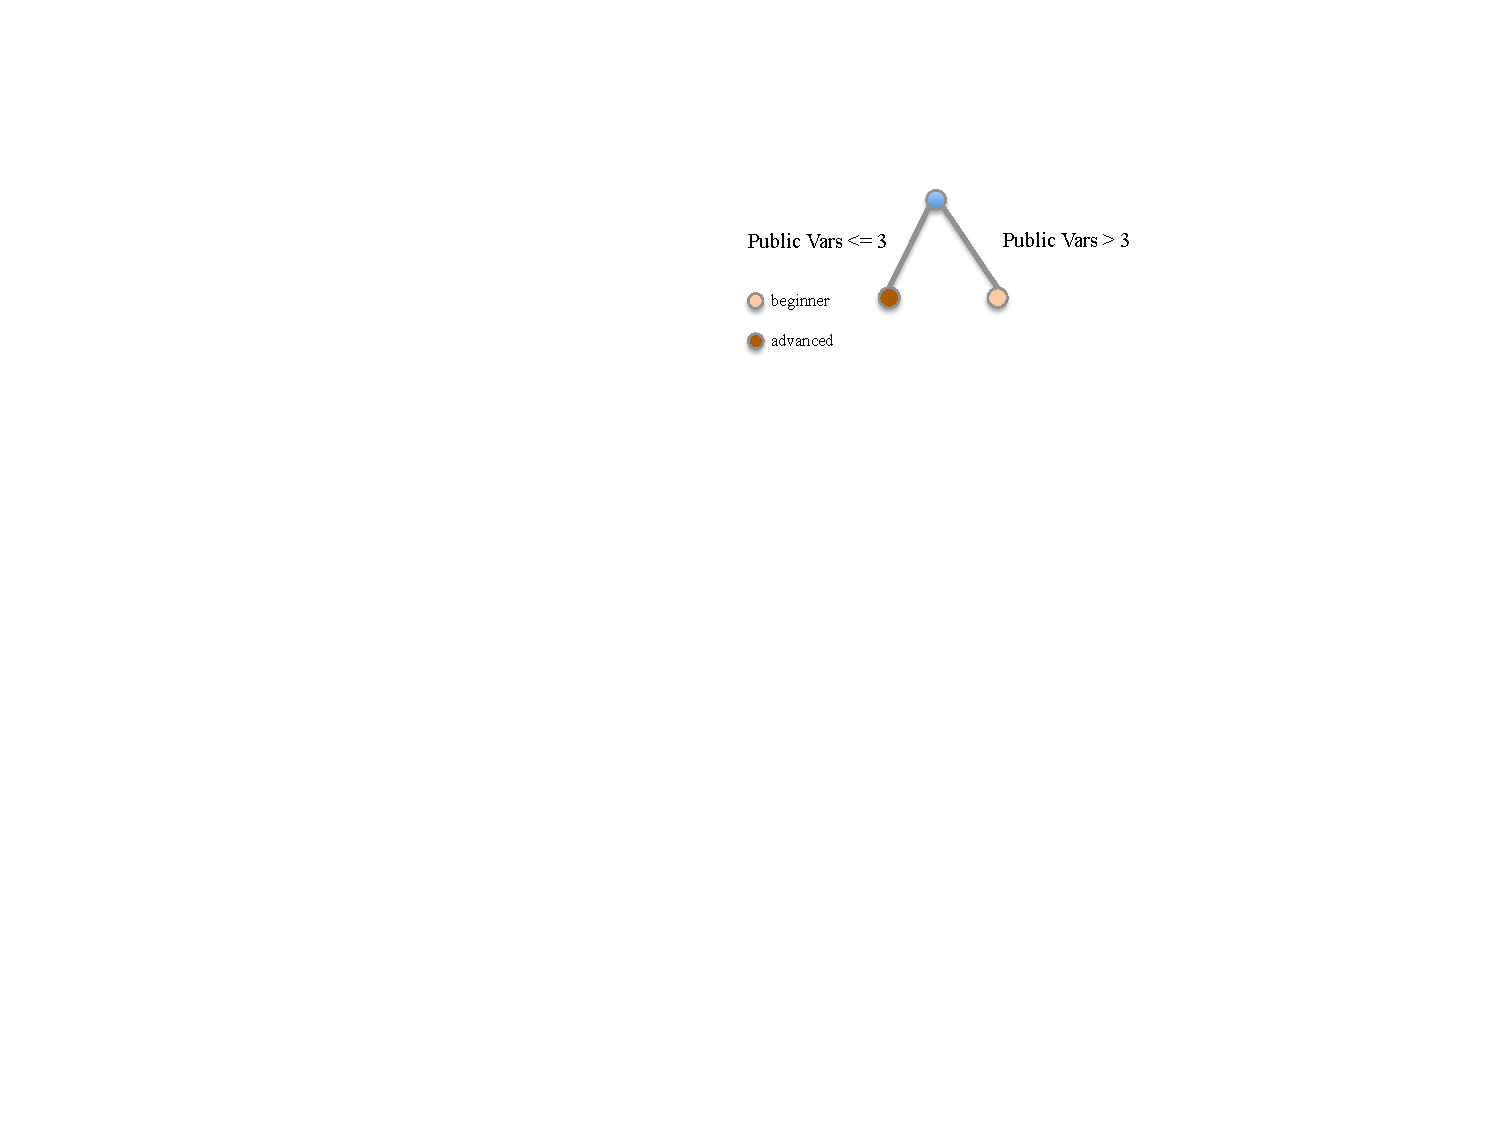
\includegraphics[width=3.5in]{Chapter-6/figs/variables.pdf}
	\caption{Variables decision tree model.}
	\label{fig:vars}
\end{figure}

\begin{figure} [h]
	\centering
	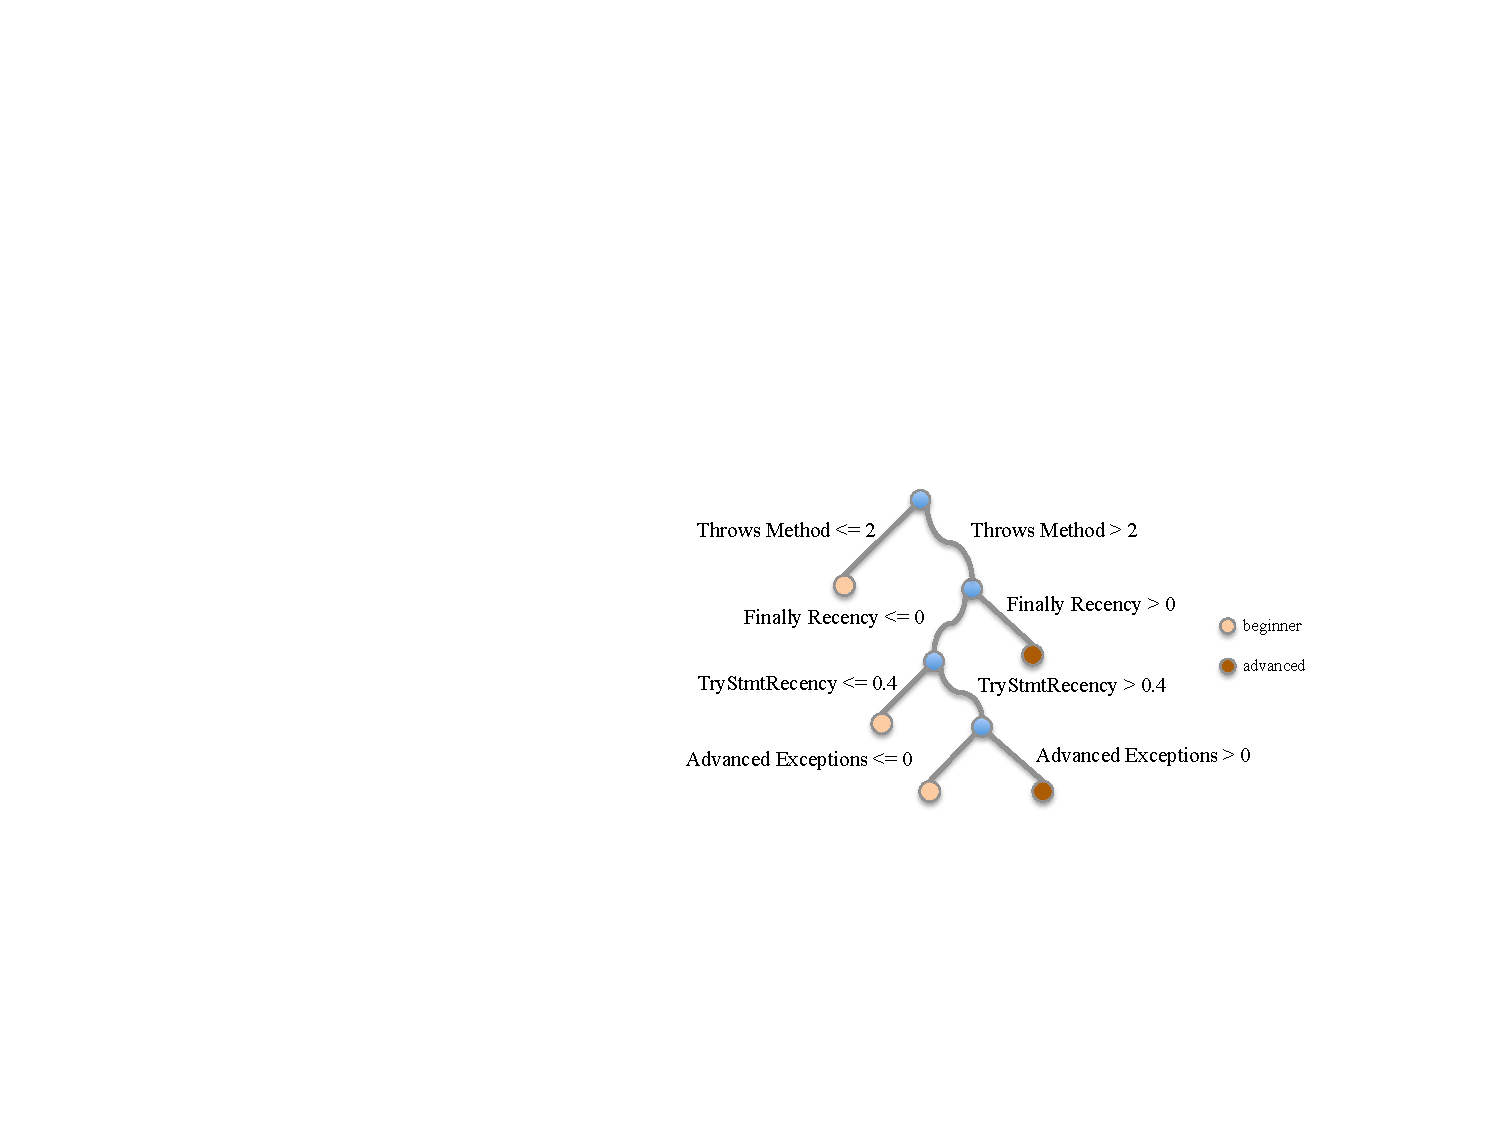
\includegraphics[width=3.5in]{Chapter-6/figs/exceptions.pdf}
	\caption{Exceptions decision tree model.}
	\label{fig:excep}
\end{figure}

\begin{figure} [h]
	\centering
	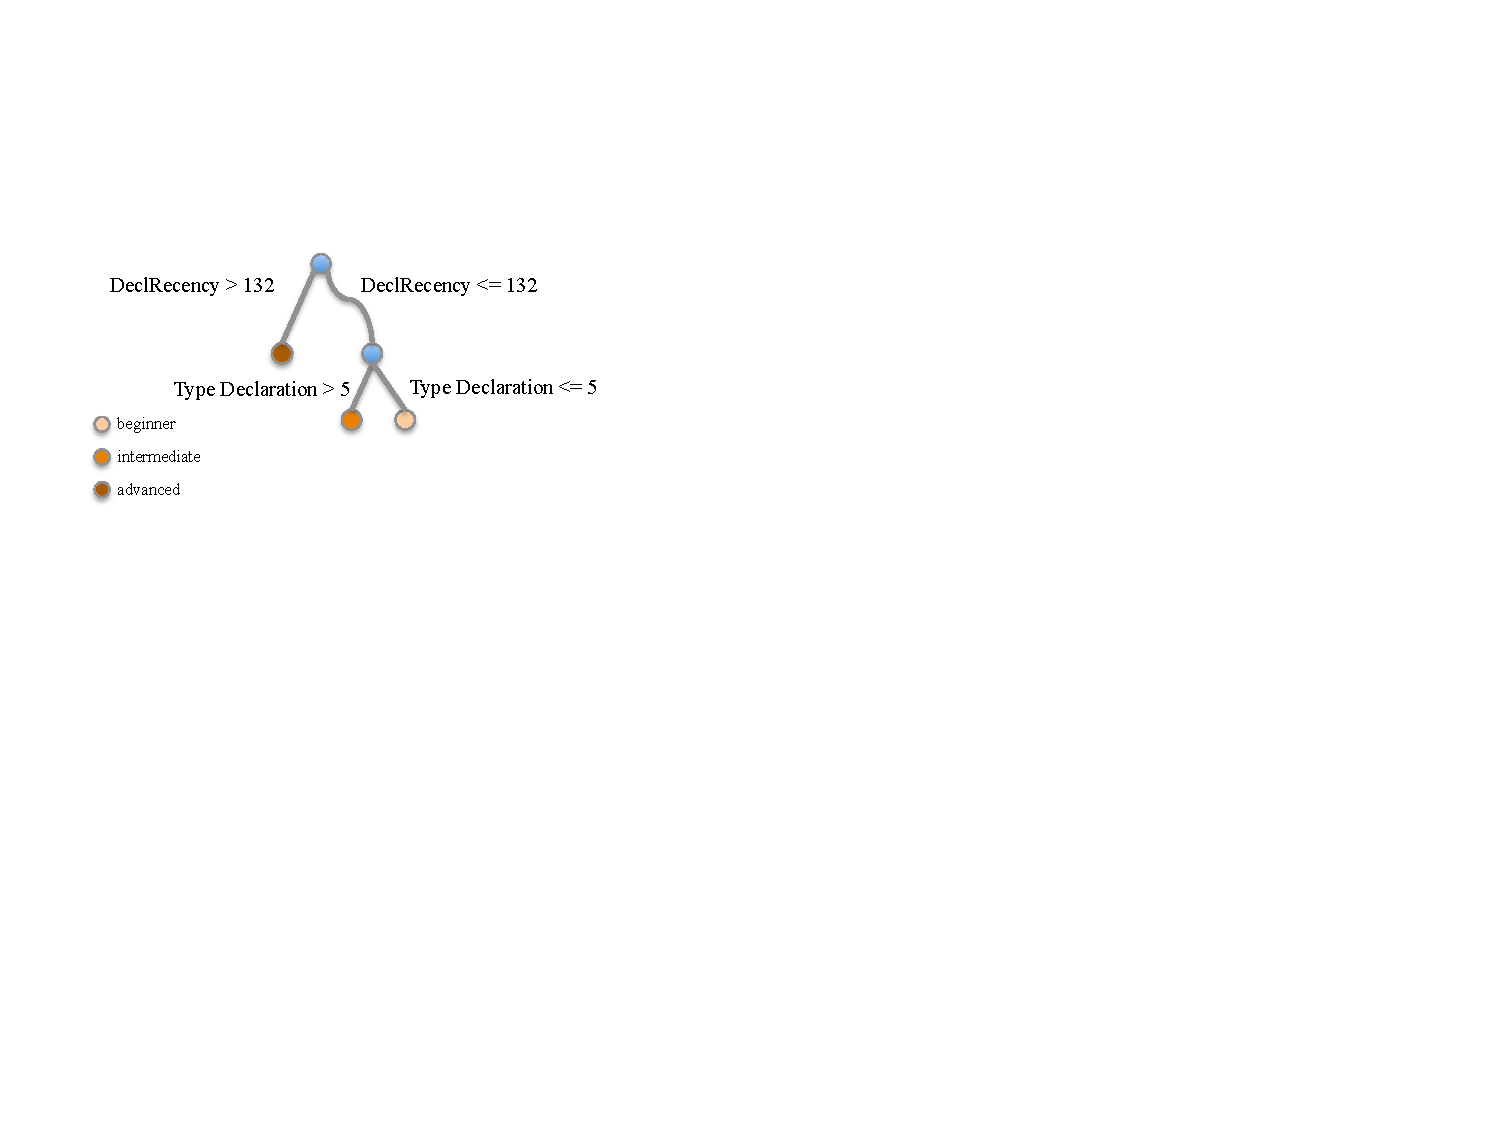
\includegraphics[width=3.5in]{Chapter-6/figs/generics.pdf}
	\caption{Generics decision tree model.}
	\label{fig:gen}
\end{figure}


\subsection{RQ\textsubscript{1} Findings}

All four decision tree models had total precision, recall, and F-Score of at least 60\%, suggesting these models correctly classified developers at least 60\% of the time. Even the model built using LOC only (Table~\ref{tab:loc}) provided accurate predictions. 
This supports existing research that suggests all of our experiences contribute to our overall knowledge~\cite{argote2011organizational}; my findings quantify this notion, showing it is possible to use developer experience to predict their knowledge.
The models also exhibit low FP rates, with a median FP rate of 19.9\%. I observed the highest FP rate with the variables model (Figure~\ref{fig:vars}); I will discuss limitations that may have caused the difference in FP rate for the variables model in Section~\ref{sec:challenges}.

Based on the attributes used in the decision trees shown in Figure~\ref{fig:gen} and Figure~\ref{fig:excep}, how recently concept-specific code was contributed can also affect conceptual knowledge. Based on the recency heuristic, for example, a higher DeclRecency (Figure~\ref{fig:gen}) value suggest more recent code contributions related to declaring generic types. This suggests that determining a developer's knowledge of generics would involve observing both declarations and recent experience with declarations. For exceptions, recency matters for some attributes, such as \texttt{try} statements and \texttt{finally} blocks, while it is not as important for others, such as usage of advanced exceptions language features. For variables, recency also did not appear to improve classification -- the variables model only includes the declaration of variables, which may have affected the ability to build an accurate and convincing model. 
% I will discuss some explanations for these results and ways to potentially improve the variables model in Section~\ref{sec:challenges}.

\vspace{1em}

\fbox{%
	\parbox{0.9\linewidth}{%
		\noindent\textbf{\textit{These findings suggest that source code can be used to classify how much developers know about programming concepts better than random chance.}}
	}%
}
\vspace{0.5em}


\subsection{RQ\textsubscript{2} Findings}

All three of the models that we trained using concept-specific attributes classified developers better than random chance ($>$ 50\%).
As for comparing the concept-specific models to a more naive model, after using CFS during data analysis, I was able to identify relevant attributes before running cross-validation during tree building. For two of the three concepts evaluated, LOC did not appear in enough folds during attribute selection to be considered during decision tree learning. Even with the variables data, which only included various attributes pertaining to variable declaration, the most meaningful attributes were concept-specific. The only data set in which LOC appeared in more than two folds was the generics data set. This suggests that in some cases, LOC is not predictive of developer concept-specific knowledge.

Upon closer examination of the generics models, overall model performance is higher in the Type Declaration model (74\%) than the LOC model (70\%), with increased precision and F-Score for beginner (\(+ 0.167\), \(+ 0.04\)) and intermediate (\(+ 0.09\), \(+ 0.1\)) classification and increased total precision (\(+ 0.05\)), recall (\(+ 0.04\)), and F-Score (\(+ 0.03\)). 
The only scenario where the LOC model outperformed the Declarations model was when classifying developers with advanced generics knowledge (Table~\ref{tab:gen}). 
These findings suggest that although both LOC and concept-specific code can both be used to predict conceptual knowledge, concept-specific code increases overall model accuracy and precision.

\vspace{1em}

\fbox{%
	\parbox{0.9\linewidth}{%
		\noindent\textit{\textbf{These findings suggest that concept-specific code improves model performance when compared to a naive model.}}
	}%
}
\vspace{0.5em}


\section{Implications}\label{sec:disc}
The ability to predict developer conceptual knowledge using attributes collected from source code opens the doors for exploring the possible applications, including the ability to adapt tool notifications to developer knowledge. 
I discuss the potential for adapting tool output and some of the other possible applications for these findings in detail below.
% Predictions for tools adaptations (building on prior work)

\subsection{Program Analysis Tool Output}
This study was motivated by the study reported in Chapter~\ref{chap:theory}, which posed a theory regarding the challenges developers encounter when attempting to understand, and eventually resolve, tool notifications~\cite{johnson2016cross}. The theory stated that the challenges developer encounter stem from gaps and mismatches between their knowledge and how tools communicate. One way to assess this theory is to explore the ability, and effectiveness, of adapting tool notifications to the knowledge of the developer using them.

% When tools communicate with developers, at the lowest, most fundamental level, they are communicating about \emph{programming-oriented concepts}, which relate to how the source code maps to programming language concepts~\cite{van2004concepts,biggerstaff1994program}. For simplicity, I refer to these concepts simply as programming concepts.
% Existing research on experience as a representation for knowledge~\cite{argote2011organizational,bromme1995fusing} and using source code contributions to predict developer knowledge of a code base~\cite{fritz2010degree} led to research questions related to using source code to predict concept-specific knowledge.

The ability to accurately classify developers' conceptual knowledge is the first step towards being able to provide meaningful notification adaptations. If a tool can automatically ascertain how much a developer knows about the concepts relevant to a given notification, it can better tailor the information provided to the information needed by that developer. The next step is to determine what a meaningful adaptation for a given developer classification looks like; this work is described in detail in Chapter~\ref{chap:improve}.

Another way that developer conceptual knowledge can be utilized by program analysis tools is to improve developers' experience when first using notifications used by the tool~\cite{johnson2015bespoke}. One of problems that have been identified with program analysis tools, especially static analysis tools, is the high volume of notifications that are sometimes presented~\cite{Johnson:2013:Why}. We can use developer conceptual knowledge to determine the notifications to prioritize. A common way current tools prioritize notifications is by problem severity, however, such strategy may not be enough to ensure a positive first experience. Also, findings from Chapter~\ref{chap:theory} suggest developers do not always agree with the prioritization used by tools~\cite{johnson2016cross}. Tools could improve the first experience by first presenting developers with notifications the tool knows they can solve based on the concepts they understand best.

\subsection{Industry \& Education Practices}
% TODO - introduce this section

For any given defect, there are one or more programming concepts relevant to understanding and being able to resolve that defect. Similar to work on code review assignment~\cite{balachandran2013reducing}, another potential application for my proposed approach for predicting conceptual knowledge is to assign the best developer to resolve a defect or complete a code review. Although knowledge of the code base is important~\cite{fritz2010degree}, my research suggests knowledge of concepts relevant to the defect or code of interest is also important~\cite{johnson2016cross}. My approach can be combined with other approaches, such as those that look at the developer's familiarity with the code base~\cite{fritz2010degree}, to assign defects to developers that are most likely to be able to resolve them. 	

The ability to predict developer knowledge also opens the door for the potential to more effectively assign  teams in industrial and educational settings. For example, if the design and implementation of a project or piece of functionality requires specific conceptual knowledge, analysis of developers' existing source code can yield information for ensuring someone with the necessary knowledge is on that team.
Along the same lines, my approach can be useful for determining effective pair programming pairs. 
Pair programming is an effective way of transferring knowledge~\cite{plonka2015knowledge} and fostering tool discovery~\cite{murphy2011peer}, both of which can aide in defect resolution. Knowledge transfer is more likely to occur when the developers paired together differ in experience (i.e. one is novice and one is expert). Furthermore, a previous study on pair programming found that the productivity provided by pair programming can drop substantially when it comes to problem solving if both programmers have experience with the problem at hand; this is especially true if the experiences are recent and has not had a chance to be forgotten~\cite{lui2006pair}. When it comes to pairing developers for a specific task, our approach can be useful for determining which developer is more expert in the concepts relevant to the task at hand. 
%~\todo{May be talk about interview screening and prep?}

\section{Lessons Learned}\label{sec:challenges}
Even with a glimpse into the possibility of modelling conceptual knowledge, there are limitations to my current approach and challenges to overcome.

% TODO think about how this is organized
\subsection{Limitations}
One limitation to my approach is that it relies solely on source code available in public repositories; not all developers have public repositories and usually not all the code a developer has written is stored in one.
Along the same lines, while analyzing developer source code can provide insights into conceptual knowledge, this may not be entirely representative of everything the developer knows about a given concept, or more importantly the notifications they encounter, which could lead to initially inaccurate models.

Another limitation to the findings presented in this chapter is that I built the models with a relatively small numbers of developers. Typically machine learning is done with large data sets, however, due to the nature of the data collected I ended up with smaller data sets (~20--30 data points). I mitigated this limitation by using decision tree learning, which has been found to work well with atypical data sets~\cite{zhang2005missing,kotsiantis2007supervised}.

One goal as I developed this approach was to provide a range of attributes relating to each concept to increase the likelihood that we are being exhaustive of relevant and possibly predictive code features. A limitation to my approach in this regard is how I dealt with a fundamental concept like variables, which can include a large range of relevant features. In this work, I decided to focus on various aspects of declaring a variable, such as data types and variable visibility, to narrow down the space of attributes being analyzed. I believe this led to the less-than-compelling model for variables conceptual knowledge found in Section~\ref{sec:eval}. Although the model is not as compelling or complex as the others, the variables model still suggests that using source code to predict concept knowledge is better than random chance or a naive model.
% not all repos 100\% Java
Another limitation is that for a small subset of developers, at least one repository was not 100\% Java. Repositories that fit into this category ranged from 42\% - 97\% Java.
Currently, my approach has only been evaluated on developers' knowledge of Java concepts, therefore a LOC model including non-Java code might have affected the results. 

\subsection{Challenges}
Mirroring the small data set limitation, one challenge to using my approach is getting enough data from the developer, especially if the developer does not have code in public repositories. One way to deal with this challenges is to modify the approach to work in on local copies and in real-time to detect developer concept-specific contributions in projects not stored in repositories.

Another challenge that comes with using my approach is determining how to deal with both fundamental and nuanced programming concepts. The findings in this chapter suggest that it may be more difficult to build an exhaustive and accurate model for fundamental concepts than it is for nuanced concepts. This may suggest that there are ways that concepts group together that can may affect how one should approach determining relevant code to collect. For example, the code we collected for variables matches the information provided on the primary sources of variables-related concepts used for the concept inventory. However, because declaring variables is necessary in most programs, there may be a need to incorporate other information such as notifications pertaining to variables the developer encountered, to get the best idea of what developers really know about variables.

Along the same lines, another challenge for my current approach is the ability to generalize across concepts. For the most exhaustive models, we can see similarities such as the fact that recency is generally important. However, it is not obvious beyond that if there is a way to general what is important to focus on when classifying developers based on their code contributions. A good starting point for work in this area would be to determine the possibility of generalizing across a subset of concepts with similar characteristics, such as splitting concepts by simple, fundamental concepts, such as variables, methods, and classes, and more complex, nuanced concepts, such as generics, exception handling, and concurrency.

% TODO more for transition here??
Despite the limitations and challenges associated with my proposed approach, the results of this study provided insights that can be used to further my research on improving the notifications tools use. In the next Chapter, I discuss how we can use developer knowledge to improve communication between developers and their tools.